% TODO: Para cada modelo colocar como que é a entrada na forma de uma expressão matemática
Este capítulo tem como objetivo apresentar uma base teórica mínima de todos os conceitos necessários para o entendimento das demais seções deste trabalho. Primeiramente, serão explicados os conceitos básicos de uma rede neural artificial e suas diferenças em relação a uma rede neural recorrente. Subsequentemente, serão explicados os conceitos principais de cada modelo utilizado neste trabalho.
\section{Tráfego}


\section{\acrfull{NN} e \acrfull{RNN}}

Redes neurais recorrentes surgiram da necessidade de avaliar os estados passados de uma rede neural para decidir sua saída atual. Redes neurais artificiais comuns, ou do tipo \textit{feedforward} precisam apenas do estímulo atual para gerar sua saída. Para exemplificar, tome como exemplo um problema de classificação, onde, a partir de uma imagem de um cachorro, ou gato, uma rede neural deva ser capaz de dizer corretamente qual animal a imagem representa. Para cada rodada de classificação, a imagem utilizada na rodada passada não importa, pois uma não tem relação direta com a outra. 

Porém, existem determinados tipos de atividades que exigem certa correlação entre os dados, como por exemplo, ler um texto, entender o contexto de um filme, avaliar a oscilação de uma bolsa de valores ao longo do tempo. Nesses exemplos, um dado isolado não tem tanto significado quanto o conjunto como um todo, o que exige um conceito de memória. Para simular este efeito de memória, redes neurais recorrentes dispõe de uma arquitetura onde a saída da célula anterior é utilizada como entrada na célula seguinte, juntamente com a entrada nova atual da rede. Abaixo pode ser visto uma fórmula com mais detalhes.

\begin{figure}[htb]
    \centering
    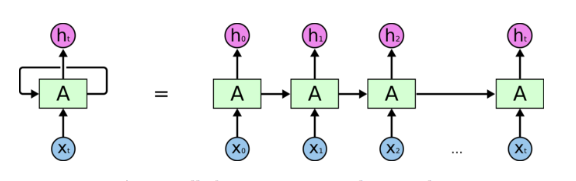
\includegraphics[scale=0.4]{rnnExample.png}
    \label{figure:eixo}
    \caption[Representação simples do conceito de um RNN]{Representação simples do conceito de uma RNN \footnotemark}
\end{figure}

\subsection{Funções de ativação}

% RESOURCE: to explain recurrent neural networks (http://d2l.ai/chapter_recurrent-neural-networks/index.html)

% TODO: Falar que nem todos os dados são independentes, então a RNN serve para lembrar de alguns dados que já passaram pelo modelo para melhorar a performance.

% TODO: Falar que é melhor para predição aparentemente (pode ser algo a ver com o tipo de dados que temos)

% TODO: Falar que sofre de memória curta e outros defeitos

% TODO?: Falar que basicamente é um modelo feito para lidar com dados dependentes

\section{\acrfull{LSTM}}

\acrshort{LSTM} é utilizado para predição de tráfego e de informações que derivam de dados sequenciais/séries temporais, sendo possível encontrar diversos trabalhos na literatura que mostram sua eficiência quando comparado a outros métodos. Como descrito em \cite{Zainab_2018} e em \cite{Xiaolei_2015}, \acrshort{LSTM} é um tipo de \acrshort{RNN} que utiliza de estados anteriores e do estado atual da rede para gerar sua saída. Ao utilizar dos estados anteriores, a \acrshort{RNN} acaba por simular uma memória, melhorando sua capacidade de aprender. 

\begin{figure}[htb]
    \centering
    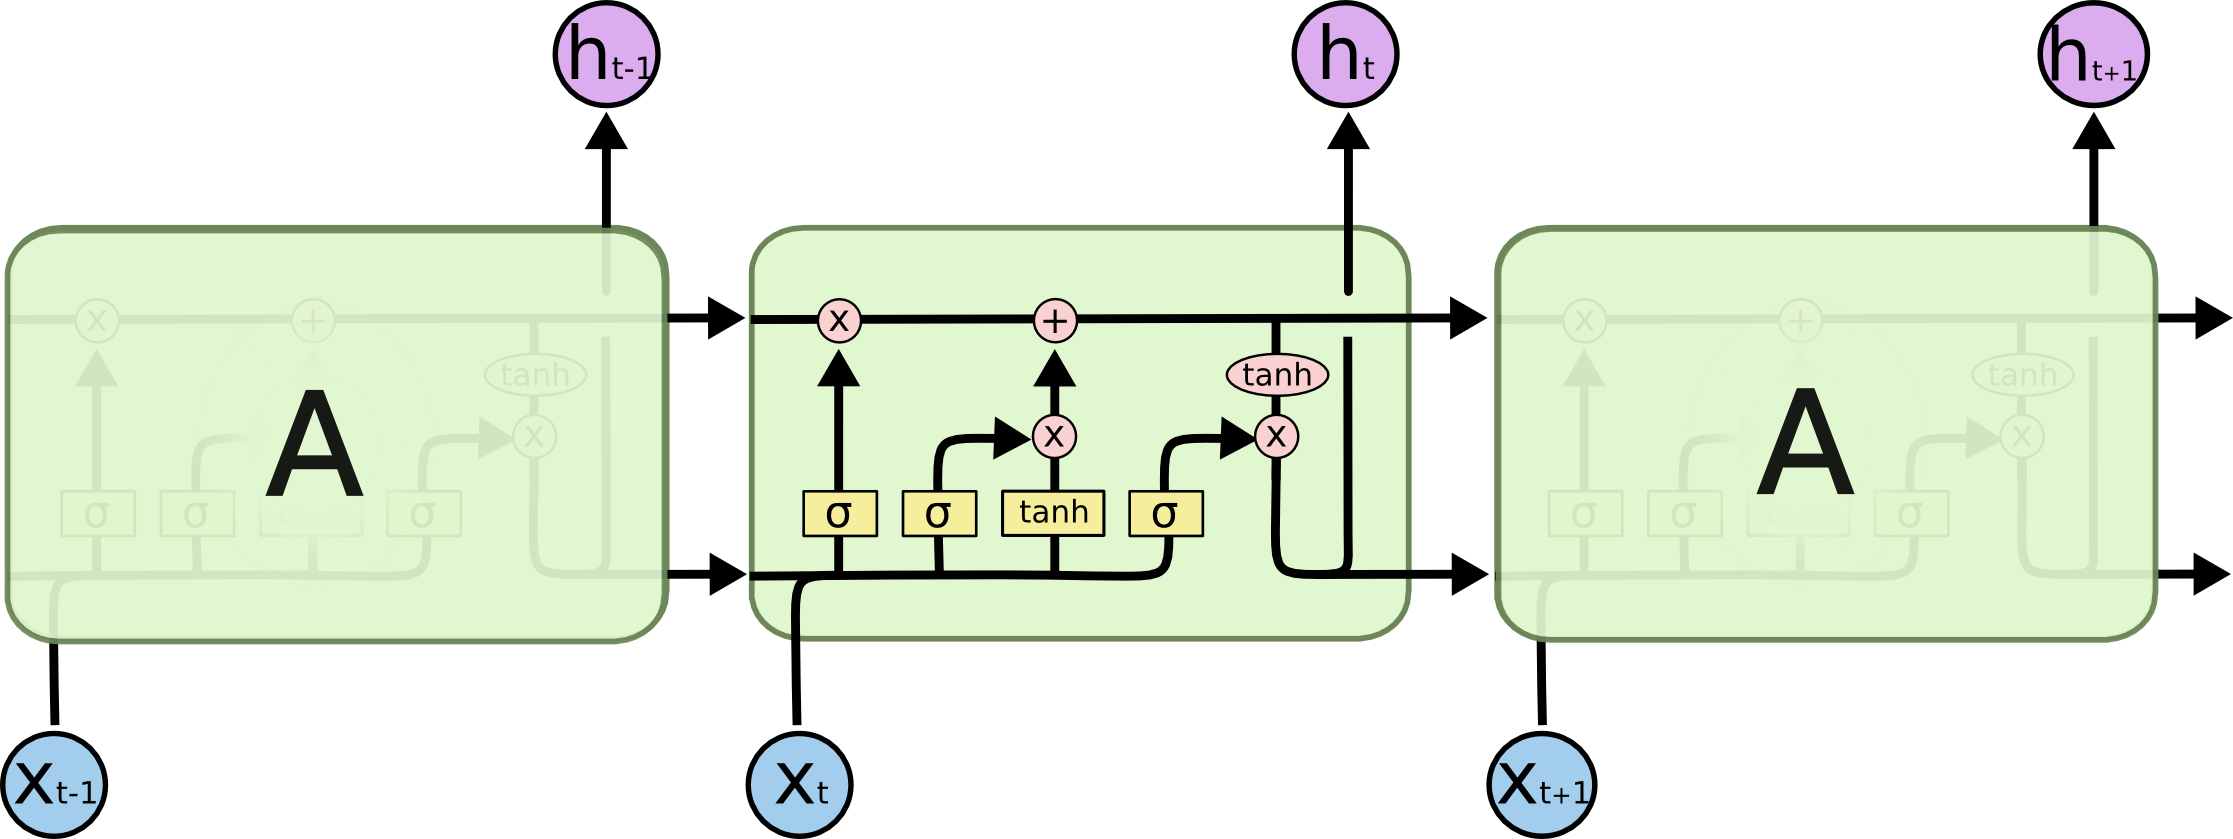
\includegraphics[scale=0.4]{lstm3.png}
    \label{figure:eixo}
    \caption[Representação de uma arquitetura LSTM]{Representação de uma arquitetura LSTM\footnotemark}
\end{figure}

\footnotetext{https://colah.github.io/posts/2015-08-Understanding-LSTMs/}

Porém, diferentemente de uma \acrshort{RNN}, o LSTM possui uma unidade a mais em seus blocos chamada de célula de memória. Esta célula é capaz de perceber as características mais latentes dos dados e descartar as menos importantes. Assim, o \acrshort{LSTM} consegue manter as características mais recorrentes na rede por mais tempo que uma \acrshort{RNN} comum. 

Na célula de memória citada anteriormente, existem estruturas que são responsáveis pela característica de memória a longo prazo do \acrshort{LSTM}. A Porta de Entrada, a Porta do esquecimento e a Porta de Saída. Abaixo está explicitado como cada um deles funciona:

\begin{itemize}
  \item Porta de Esquecimento: A primeira porta de uma célula do \acrfull{LSTM} decide qual informação provinda da célula anterior vai ser descartada. Isso é feito por meio de uma função de ativação sigmoidal que retorna um número entre 0 e 1 para cada valor da célula passada, onde 0 representa total esquecimento daquela informação e 1 total preservação.
  
  \item Porta do Entrada: A segunda porta decide qual informação deve ser atualizada. Para tal decisão são utilizadas duas funções. Primeiro, uma função sigmoid decide quais valores serão atualizados. Depois uma função Tahn cria novos valores candidatos a serem utilizados na atualização.
  \item Porta de Saída:
\end{itemize}

% TODO: Falar que podemos responder a quantidade de camadas da LSTM com o problema que RNN tem com back-propagation que o gradiente começa a diminuir exponencialmente. Mas tem que dar uma conferida melhor.

\section{\acrfull{GRU}}

\acrofull{GRU} é um tipo de \acrofull{RNN} semelhante ao \acrofull{LSTM}, porém, mais simples. Sua arquitetura consiste em:

\begin{itemize}
    \item 
    \item
    \item
\end{itemize}

\section{Árvores de Decisão}

% TODO: talk abiut overfitting

Árvores de decisão sobre-ajustam muito fácil no conjunto de dados por ser muito flexível e poderoso, memorizando parte do conjunto de dados. Podendo, por exemplo, criar uma árvore que cada folha corresponde a somente um elemento.

% https://towardsdatascience.com/an-implementation-and-explanation-of-the-random-forest-in-python-77bf308a9b76
 Algoritmos podem ser flexíveis e correr risco de sobre-ajuste ou ser inflexíveis e não conseguir se ajustar nos dados. Modelos flexiveis demais podem  meomorizar os dados e modelos inflexiveis presupõe informações sobre os dados.
 Árvore de decisão é flexível se não for limitar o tamanho da árvore e inflexível se vc limitar demais o tamanho da árvore. Isso é chamado de bias-variance tradeof.
 
\begin{figure}[h]
    \centering
    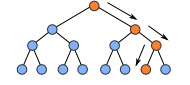
\includegraphics[scale=1.5]{monography/img/decision_tree.png}
    \label{figure:rf}
    \caption{Representação do funcionamento de uma Árvore de Decisão\footnotemark}
\end{figure}

\footnotetext{Corte de uma imagem de uma \textit{\acrshort{RF}} https://dsc-spidal.github.io/harp/img/4-5-1.png}

\section{\acrfull{RF}}

% TODO: checar se a tradução está correta (frase pega do abstract do artigo)
Criado por Leo Breiman em \textit{Random Forest} \cite{Breiman:2001:RF:570181.570182}, \textit{\acrshort{RF}} é um método de aprendizagem de máquina utilizado tanto para classificação quanto para regressão. Segundo o autor, o método é uma combinação de árvores de decisão onde cada árvore de decisão depende de uma amostra aleatória independente do conjunto de dados e que todas as árvores de decisão tenham a mesma distribuição. 

Mais especificamente, a construção das árvores de decisão são feitas utilizando do método \textit{Bagging} (\textit{\textbf{B}ootstrap \textbf{Agg}regation}) criado por Leo Breiman em \textit{Bagging Predictors} \cite{Breiman:1996:BP:231986.231989}. Este método gera várias versões de um mesmo modelo e agrega os resultados dos mesmos. As versões do modelo utilizam réplicas do conjunto de dados com a mesma distribuição e com apenas uma parte do mesmo selecionada de forma aleatória.

Porém, diferente de \textit{Bagging}, \textit{\acrshort{RF}} utiliza de mais uma técnica para diminuir o sobre-ajuste (\textit{overfitting}). Há uma modificação no algoritmo de criação das árvores de decisão limitando a quantidade de características (\textit{features}) do conjunto de dados que vai ser utilizado. Para selecionar a quantidade ideal de características o autor sugere utilizar de estimativas \textit{out-of-bag}, mas é comum implementações limitarem a quantidade de características (\textit{q}) para $ \sqrt{q} $ ou $ \frac{q}{3} $.

Como \textit{\acrshort{RF}} é uma combinação de outros modelos de aprendizagem de máquina, este pode ser classificado como um Comitê de Máquinas (\textit{Ensemble Learning}). A forma como as respostas de cada uma das máquinas são combinadas depende do problema, para classificação pode ser usado uma votação (voto da maioria) e para um problema de regressão pode ser usado uma média dos valores, assim como mostrado na Figura \ref{figure:rf}.

\begin{figure}[h]
    \centering
    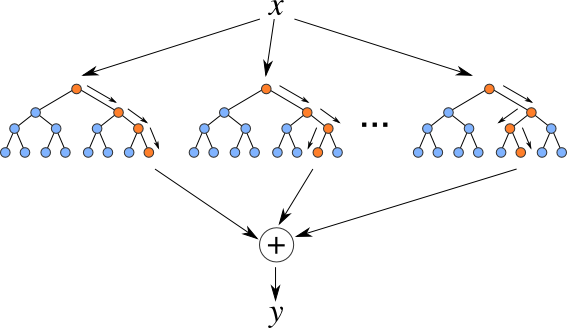
\includegraphics[scale=0.8]{monography/img/random_forest.png}
    \label{figure:rf}
    \caption{Representação do funcionamento de uma \textit{\acrshort{RF}}\footnotemark}
\end{figure}

\footnotetext{https://dsc-spidal.github.io/harp/img/4-5-1.png}

% RESOURCE: to learn better how random forest work (https://stackabuse.com/random-forest-algorithm-with-python-and-scikit-learn/)

\section{\acrfull{SVM}}

\textit{\acrshort{SVM}} foi criado originalmente por Vapnik nos anos 60 e foi evoluindo até se tornar o que é hoje, segundo Smola et. al. \cite{Smola03atutorial}. A ideia básica por trás do método pode ser usada tanto para classificação quanto para regressão. 

No caso da regressão, tenta-se criar uma função  de forma que se \(y(x)\) é a função que perfeitamente descreve o conjunto de dados e \(\epsilon\) seja a dimensão do erro, o ideal seria \(\abs{y(x) - f(x)} \leq \epsilon \)

Além disso, é SVM possui um truque chamado "kernel trick", esse truque é utilizado para mudar a dimensão do pontos de forma a representar o dataset em outra dimensão. Permitindo trabalhar melhor

Além disso, SVM possuem "kernels", isto é, funções que mudam a dimensão da entrada. 

Funções kernel são responsáveis por mapear entradas em uma dimensão para outras. Podendo essa outra ser uma dimensão superior a entrada. Isso é útil caso o conjunto de dados esteja uma dimensão que é difícil criar uma função resolva a equação.

O kernel trick é a capacidade de fazer as transformações das entradas de forma mais eficiente.

Dependendo do kernel, pode levar a overfitting

Variável C indica quanto os erros penalizam. Se for baixo, erros não serão mt penalizados e se for alto os erros serão mt penalizados

Variável Gamma é uma variável do kernel que ajuda a controlar o bias variance tradeoff. Valores baixos de Gamma podem resultar em

Variável Gamma diz quanto de influência os suport vector tem uma alta influência na classificação de um próximo elemento de uma forma inversamente proporcional. Quanto maior o valor, menor a influência do support vector, quanto menor o valor, maior o influenciaml. Valores baixos pode levar a um bias alto e variância baixa, prono a . Já valores altos podem levar a um boas baixo e variância alta, prono a overfitting.

Gamma é inversamente proporcional a bias e diretamente proporcional a variaca

Nem todo kernel tem a variável Gamma, na implementação utilizada no trabalho somente os kernels rbf, poly e sigmoid 
Reference: https://scikit-learn.org/stable/modules/generated/sklearn.svm.SVR.html




Existem várias funções kernel como linear, não linear, radial basis function, polinomial,, entre outros

+ Vou precisar falar do boas variavnce tradeoff para explicar Gamma

% TODO: explicar como ele é lerdo para tamanhos mt grandes já que ele tende a ser cúbico
% TODO: parece que ele pode overfitar com um grande número de features
% TODO: explicar um pouco como funciona o Kernel
% TODO: falar sobre como funciona o parâmetro C
% TODO: falar sobre como funciona o parâmetro Gamma

\begin{figure}[h]
    \centering
    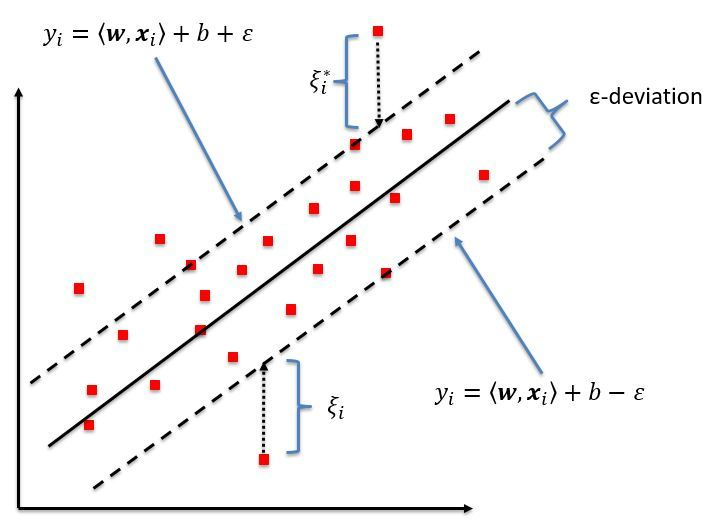
\includegraphics[scale=1.0]{monography/img/svr_example.png}
    \label{figure:rf}
    \caption{Representação do funcionamento de uma Árvore de Decisão\footnotemark}
\end{figure}

\footnotetext{https://www.researchgate.net/figure/Schematic-of-the-one-dimensional-support-vector-regression-SVR-model-Only-the-points_fig5_320916953}


